\begin{figure}[H]
    \centering

\begin{tikzpicture}
\pgfplotsset{
    every axis/.style={ymin=0},
    width=0.75\textwidth,
    height=0.25\textheight,
    xtick={1, 2, 3, 4, 5, 6, 7, 8},
    y axis style/.style={
    yticklabel style=#1,
    ylabel style=#1,
    y axis line style=#1,
    ytick style=#1}}
\begin{axis}[ scale only axis, ymin=0, ymax=170, xmin=1,xmax=8, axis y line*=left, xlabel=Number of Cores, ylabel=Execution time (s), y axis style=green!75!black]
    \addplot[smooth, green!75!black, mark=o, draw] 
    coordinates 
    {
        (1,146)
        (2,95)
        (3,78)
        (4,70)
        (5,68)
        (6,65)
        (7,63)
        (8,61)
    };
\end{axis}
%
\begin{axis}[ scale only axis, ymin=0, ymax=1800, xmin=1,xmax=8, axis y line*=right, axis x line=none, ylabel=DEC (j), y axis style=blue]%
    \addplot[smooth, blue, mark=x] 
    coordinates 
    {
        (1,858)
        (2,934)
        (3,945)
        (4,1096)
        (5,1098)
        (6,1077)
        (7,1074)
        (8,1063)
    };
\end{axis}
%
\begin{axis}[red, scale only axis, ymin=0, ymax=20, xmin=1,xmax=8, axis y line*=right, axis x line=none, ylabel=DEC per second (w)]%
\pgfplotsset{every outer y axis line/.style={xshift=2cm}, every tick/.style={xshift=2cm}, every y tick label/.style={xshift=2cm} }
    \addplot[smooth, red ,mark=+] 
    coordinates 
    {
        (1,5.850602)
        (2,9.453369)
        (3,11.57187)
        (4,14.817151)
        (5,15.37859)
        (6,15.7297)
        (7,16.1356)
        (8,16.4475)
    };
\end{axis} 

\end{tikzpicture}
    \caption{The evolution of the DEC (blue), DEC per second (red) and execution time (green) as more cores are allocated to 3DM on DUT 1}
    \label{fig:exp_3_dut_1_3dm_result}
\end{figure}